\documentclass[final,t,serif]{beamer}\usepackage[]{graphicx}\usepackage[]{color}
%% maxwidth is the original width if it is less than linewidth
%% otherwise use linewidth (to make sure the graphics do not exceed the margin)
\makeatletter
\def\maxwidth{ %
  \ifdim\Gin@nat@width>\linewidth
    \linewidth
  \else
    \Gin@nat@width
  \fi
}
\makeatother

\definecolor{fgcolor}{rgb}{0.345, 0.345, 0.345}
\newcommand{\hlnum}[1]{\textcolor[rgb]{0.686,0.059,0.569}{#1}}%
\newcommand{\hlstr}[1]{\textcolor[rgb]{0.192,0.494,0.8}{#1}}%
\newcommand{\hlcom}[1]{\textcolor[rgb]{0.678,0.584,0.686}{\textit{#1}}}%
\newcommand{\hlopt}[1]{\textcolor[rgb]{0,0,0}{#1}}%
\newcommand{\hlstd}[1]{\textcolor[rgb]{0.345,0.345,0.345}{#1}}%
\newcommand{\hlkwa}[1]{\textcolor[rgb]{0.161,0.373,0.58}{\textbf{#1}}}%
\newcommand{\hlkwb}[1]{\textcolor[rgb]{0.69,0.353,0.396}{#1}}%
\newcommand{\hlkwc}[1]{\textcolor[rgb]{0.333,0.667,0.333}{#1}}%
\newcommand{\hlkwd}[1]{\textcolor[rgb]{0.737,0.353,0.396}{\textbf{#1}}}%

\usepackage{framed}
\makeatletter
\newenvironment{kframe}{%
 \def\at@end@of@kframe{}%
 \ifinner\ifhmode%
  \def\at@end@of@kframe{\end{minipage}}%
  \begin{minipage}{\columnwidth}%
 \fi\fi%
 \def\FrameCommand##1{\hskip\@totalleftmargin \hskip-\fboxsep
 \colorbox{shadecolor}{##1}\hskip-\fboxsep
     % There is no \\@totalrightmargin, so:
     \hskip-\linewidth \hskip-\@totalleftmargin \hskip\columnwidth}%
 \MakeFramed {\advance\hsize-\width
   \@totalleftmargin\z@ \linewidth\hsize
   \@setminipage}}%
 {\par\unskip\endMakeFramed%
 \at@end@of@kframe}
\makeatother

\definecolor{shadecolor}{rgb}{.97, .97, .97}
\definecolor{messagecolor}{rgb}{0, 0, 0}
\definecolor{warningcolor}{rgb}{1, 0, 1}
\definecolor{errorcolor}{rgb}{1, 0, 0}
\newenvironment{knitrout}{}{} % an empty environment to be redefined in TeX

\usepackage{alltt}
\mode<presentation>
{
%  \usetheme{Warsaw}
%  \usetheme{Aachen}
%  \usetheme{Oldi6}
%  \usetheme{I6td}
  \usetheme{I6dv}
%  \usetheme{I6pd}
%  \usetheme{I6pd2}
}
% additional settings
\setbeamerfont{itemize}{size=\normalsize}
\setbeamerfont{itemize/enumerate body}{size=\normalsize}
\setbeamerfont{itemize/enumerate subbody}{size=\normalsize}

% additional packages
\usepackage{xcolor}
\usepackage{amsmath,amsthm, amssymb, latexsym}
\usepackage{exscale}
\usepackage{subfig}
%\boldmath
\usepackage{booktabs, array}
\usepackage{tabularx}
%\usepackage{rotating} %sideways environment
\usepackage[english]{babel}
\usepackage[latin1]{inputenc}
\usepackage{times}
\usepackage[orientation=landscape,size=custom,width=115.57,height=99.695,scale=1.55]{beamerposter} % in cm, equal to 45.5" wide x 39.3701" high
\listfiles
% Display a grid to help align images
%\beamertemplategridbackground[1cm]

\newcolumntype{R}{>{\raggedleft\arraybackslash}X}


\title{\LARGE Trend analysis of four decades of water quality data in the upper San Francisco Estuary}
\author[Beck et al.]{Marcus W. Beck\textsuperscript{1}, David Senn, Emily Novick, Phil Bresnahan, James D. Hagy III, Thomas Jabusch}
\institute[USEPA GED]{\textsuperscript{1}US Environmental Protection Agency ORD NHEERL, Gulf Ecology Division, Gulf Breeze, FL}
\date[April 20, 2016]{April 20, 2016}



\IfFileExists{upquote.sty}{\usepackage{upquote}}{}
\begin{document}

\begin{frame}{}

	\vspace{-0.6cm} %spacing for block distance from header
  \begin{columns}[t]
  	\hspace{0.4cm}
  	
  	%%%%%%%%%%%%%%
  	% LEFT
  	%%%%%%%%%%%%%%
  	\begin{column}{.31\linewidth}

			%%%%%%
			% abstract
			%%%%%%
      \begin{block}{Abstract}
        		\alert{\small Recent methods for trend analysis have been developed that leverage the descriptive potential of long term time series.  Combined with these methods, multi-decadal datasets of water quality in the San Francisco Estuary (SFE) could provide a valuable opportunity to gain insight into ecosystem properties and drivers of change in estuaries.  This study explores the use of an estuarine adaptation of the Weighted Regression on Time, Discharge, and Season (WRTDS) approach to describe nutrient trends in the northern region of SFE (Suisun Bay and the Delta), a primary source of nutrients into the system.  This novel technique is data-driven where the parameterization of the functional model changes smoothly over time following dynamic patterns of season and flow.  By doing so, changes over time that have not been previously quantified can be described, including variation in flow-normalized concentrations, frequency occurrence of extreme events, and response to historical changes in the watershed, all of which are important needs for understanding trends in the northern SFE.  The goal of the analysis is to apply the WRTDS model at multiple stations in the Delta and Suisun Bay regions of SFE to describe variation over time and relationships between key species of dissolved inorganic nitrogen (ammonium, nitrate/nitrite, total).  This variation is considered in the context of varying contributions of input flows from the Sacramento and San Joaquin rivers, as well as tidal exchange with the central SFE.  Overall, this analysis is expected to further an ecological and management-based understanding of dynamics in SFE, with implications for water quality restoration and protection of this prominent system.}
      \end{block}
      
      %%%%%%
      % Objectives
      %%%%%%
      \begin{block}{Analysis components}
    	\begin{itemize}
    	\item WRTDS trend analysis method applied to \alert{nine stations} in SFE
    	\item Models were developed for three \alert{nitrogen analytes} 
    	\item Results were evaluated as \alert{flow-normalized trends}
    	\end{itemize}
    	
      \end{block}
      		
      %%%%%%
      % Data
      %%%%%%

			\begin{block}{Data and WRTDS model}
	    Nine nutrient stations with bimonthly samples and daily flow estimates from major inflows
	    
	    \begin{figure}
      \centerline{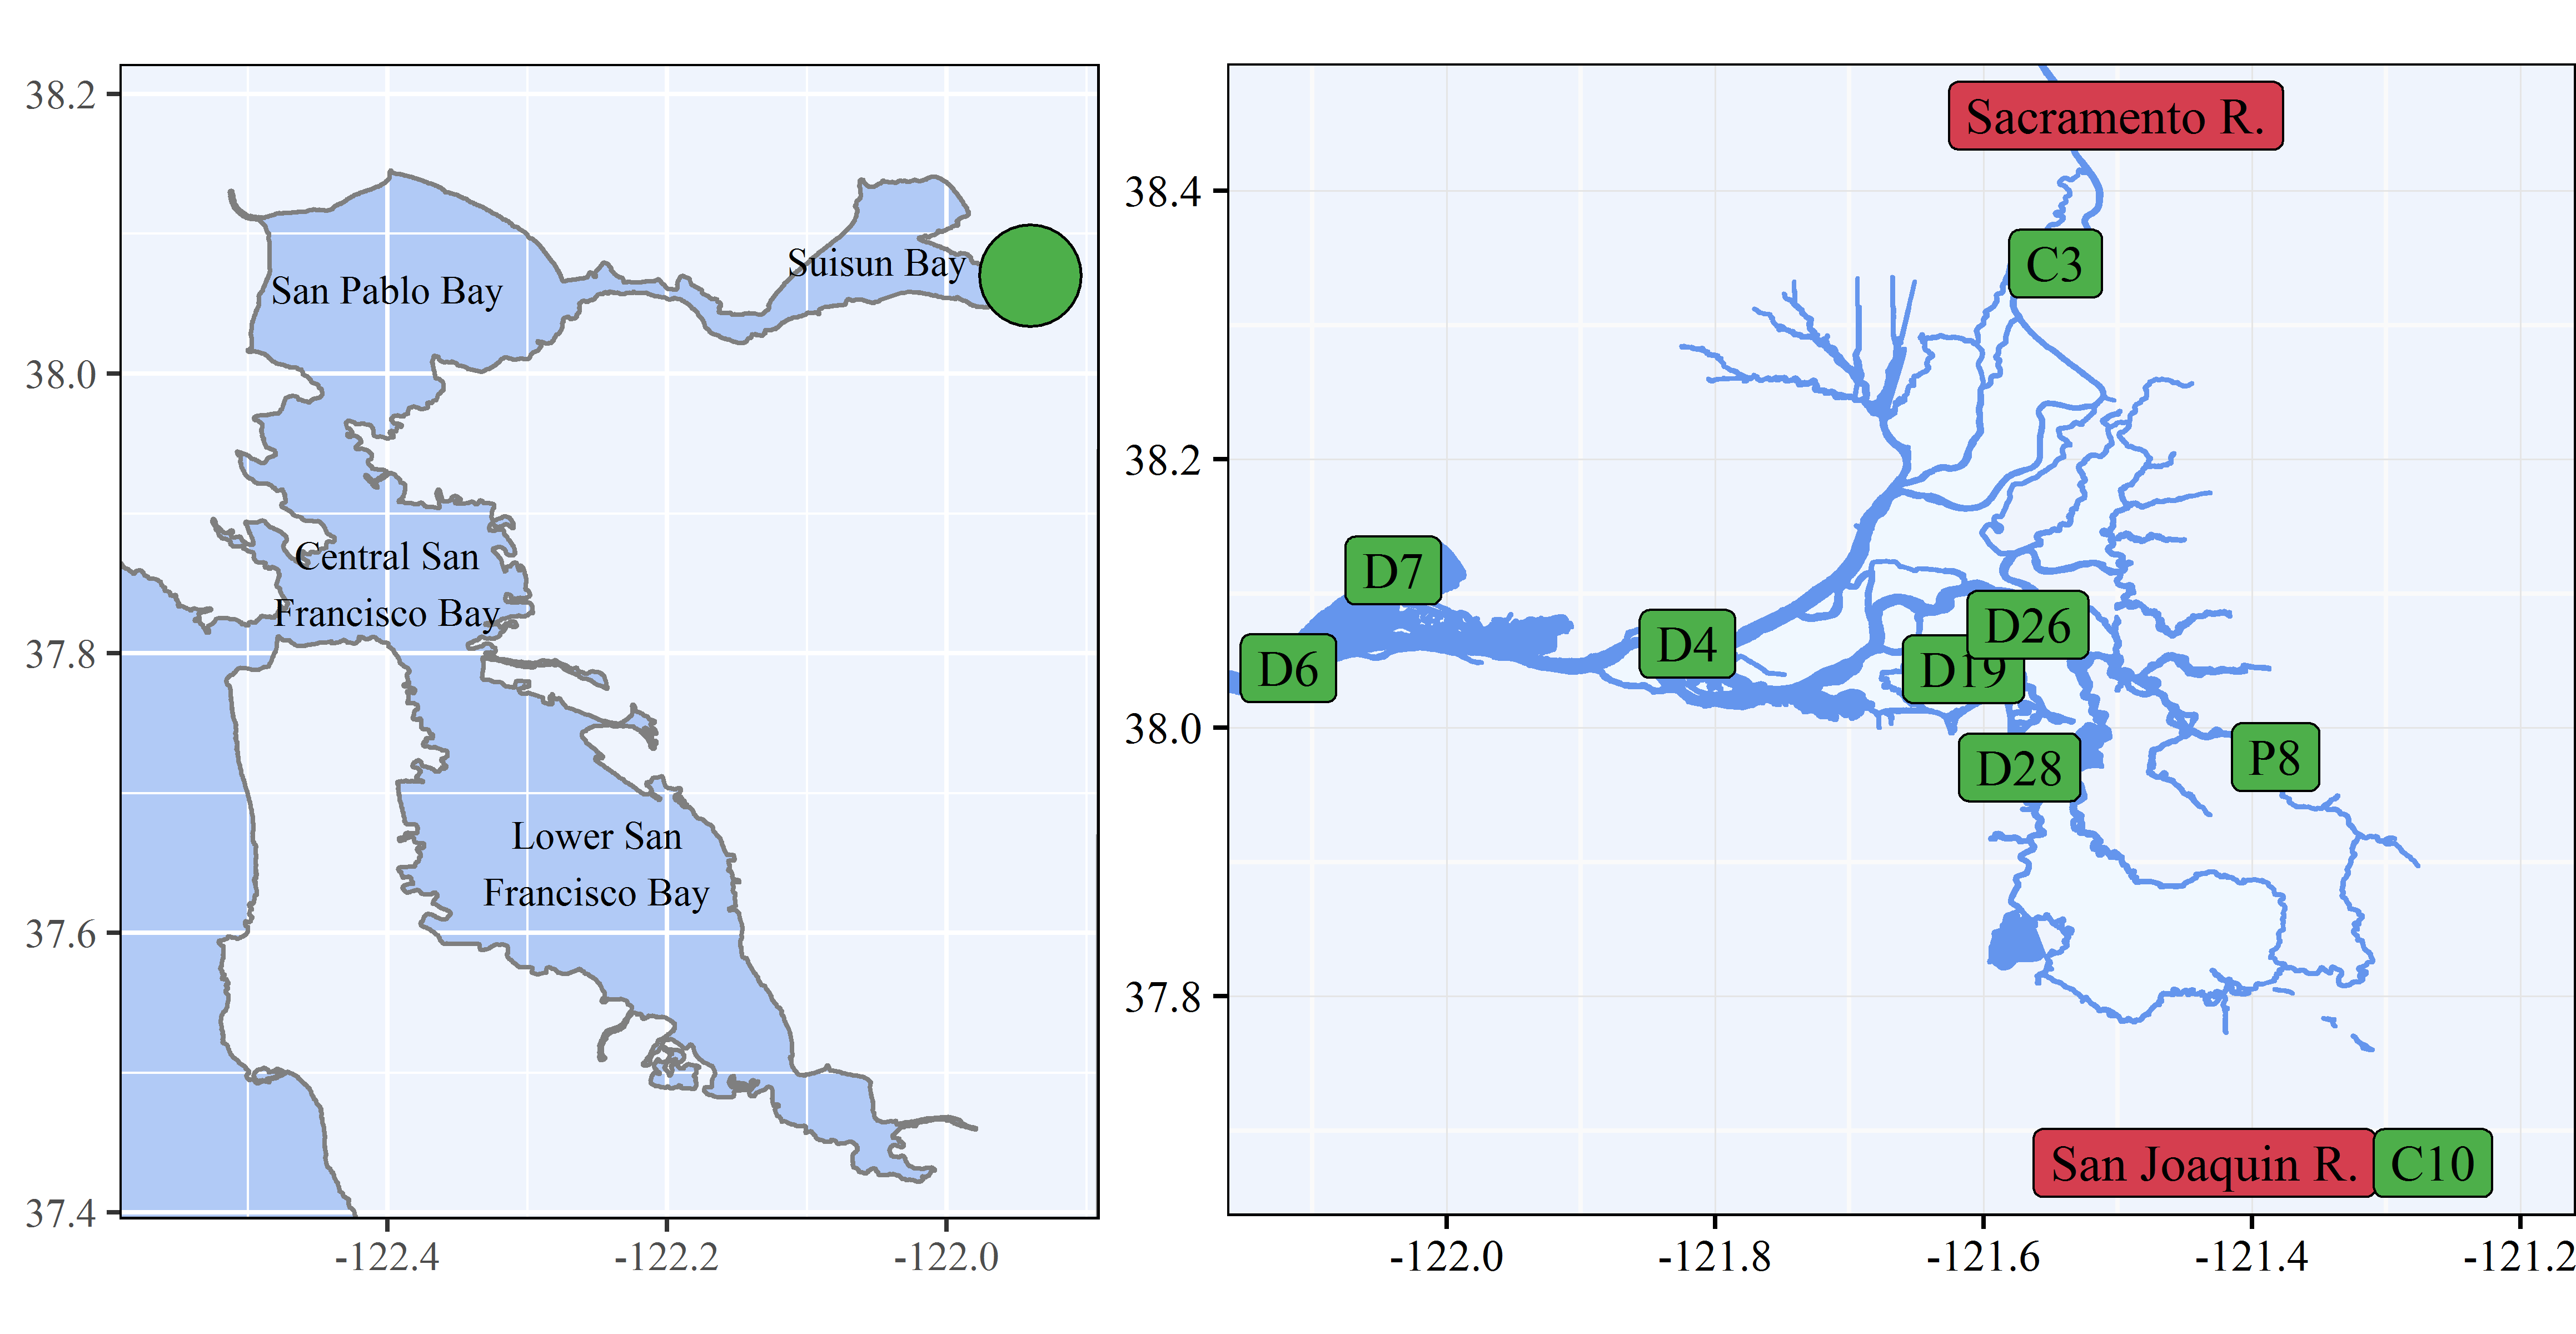
\includegraphics[width=0.75\linewidth]{posterfigs/stations.png}}
      \caption{\footnotesize Locations of nutrient stations in SFE, sampled bimonthly.}
	    \end{figure}
	    \vspace{-1.5cm}
	    WRTDS models for DIN, NO$_{2}^{-}$/NO$_{3}^{2-}$, NH$_{4}^{2+}$
			\end{block}

    \end{column}
    
  	%%%%%%%%%%%%%%
  	% CENTER
  	%%%%%%%%%%%%%%    
    \begin{column}{.62\linewidth}

    
      %%%%%%
      % model application
      %%%%%%
      \begin{block}{Model Applications}
      
      \begin{columns}
      
      \begin{column}{0.45\linewidth}
      \small
      \centerline{$\ln\left(N\right) = \beta_0 + \beta_1 t + \beta_2 \ln\left(Q\right) + \beta_3 \sin\left(2\pi t\right) + \beta_4 \cos\left(2\pi t\right) + \epsilon$}
	    \begin{figure}
      \centerline{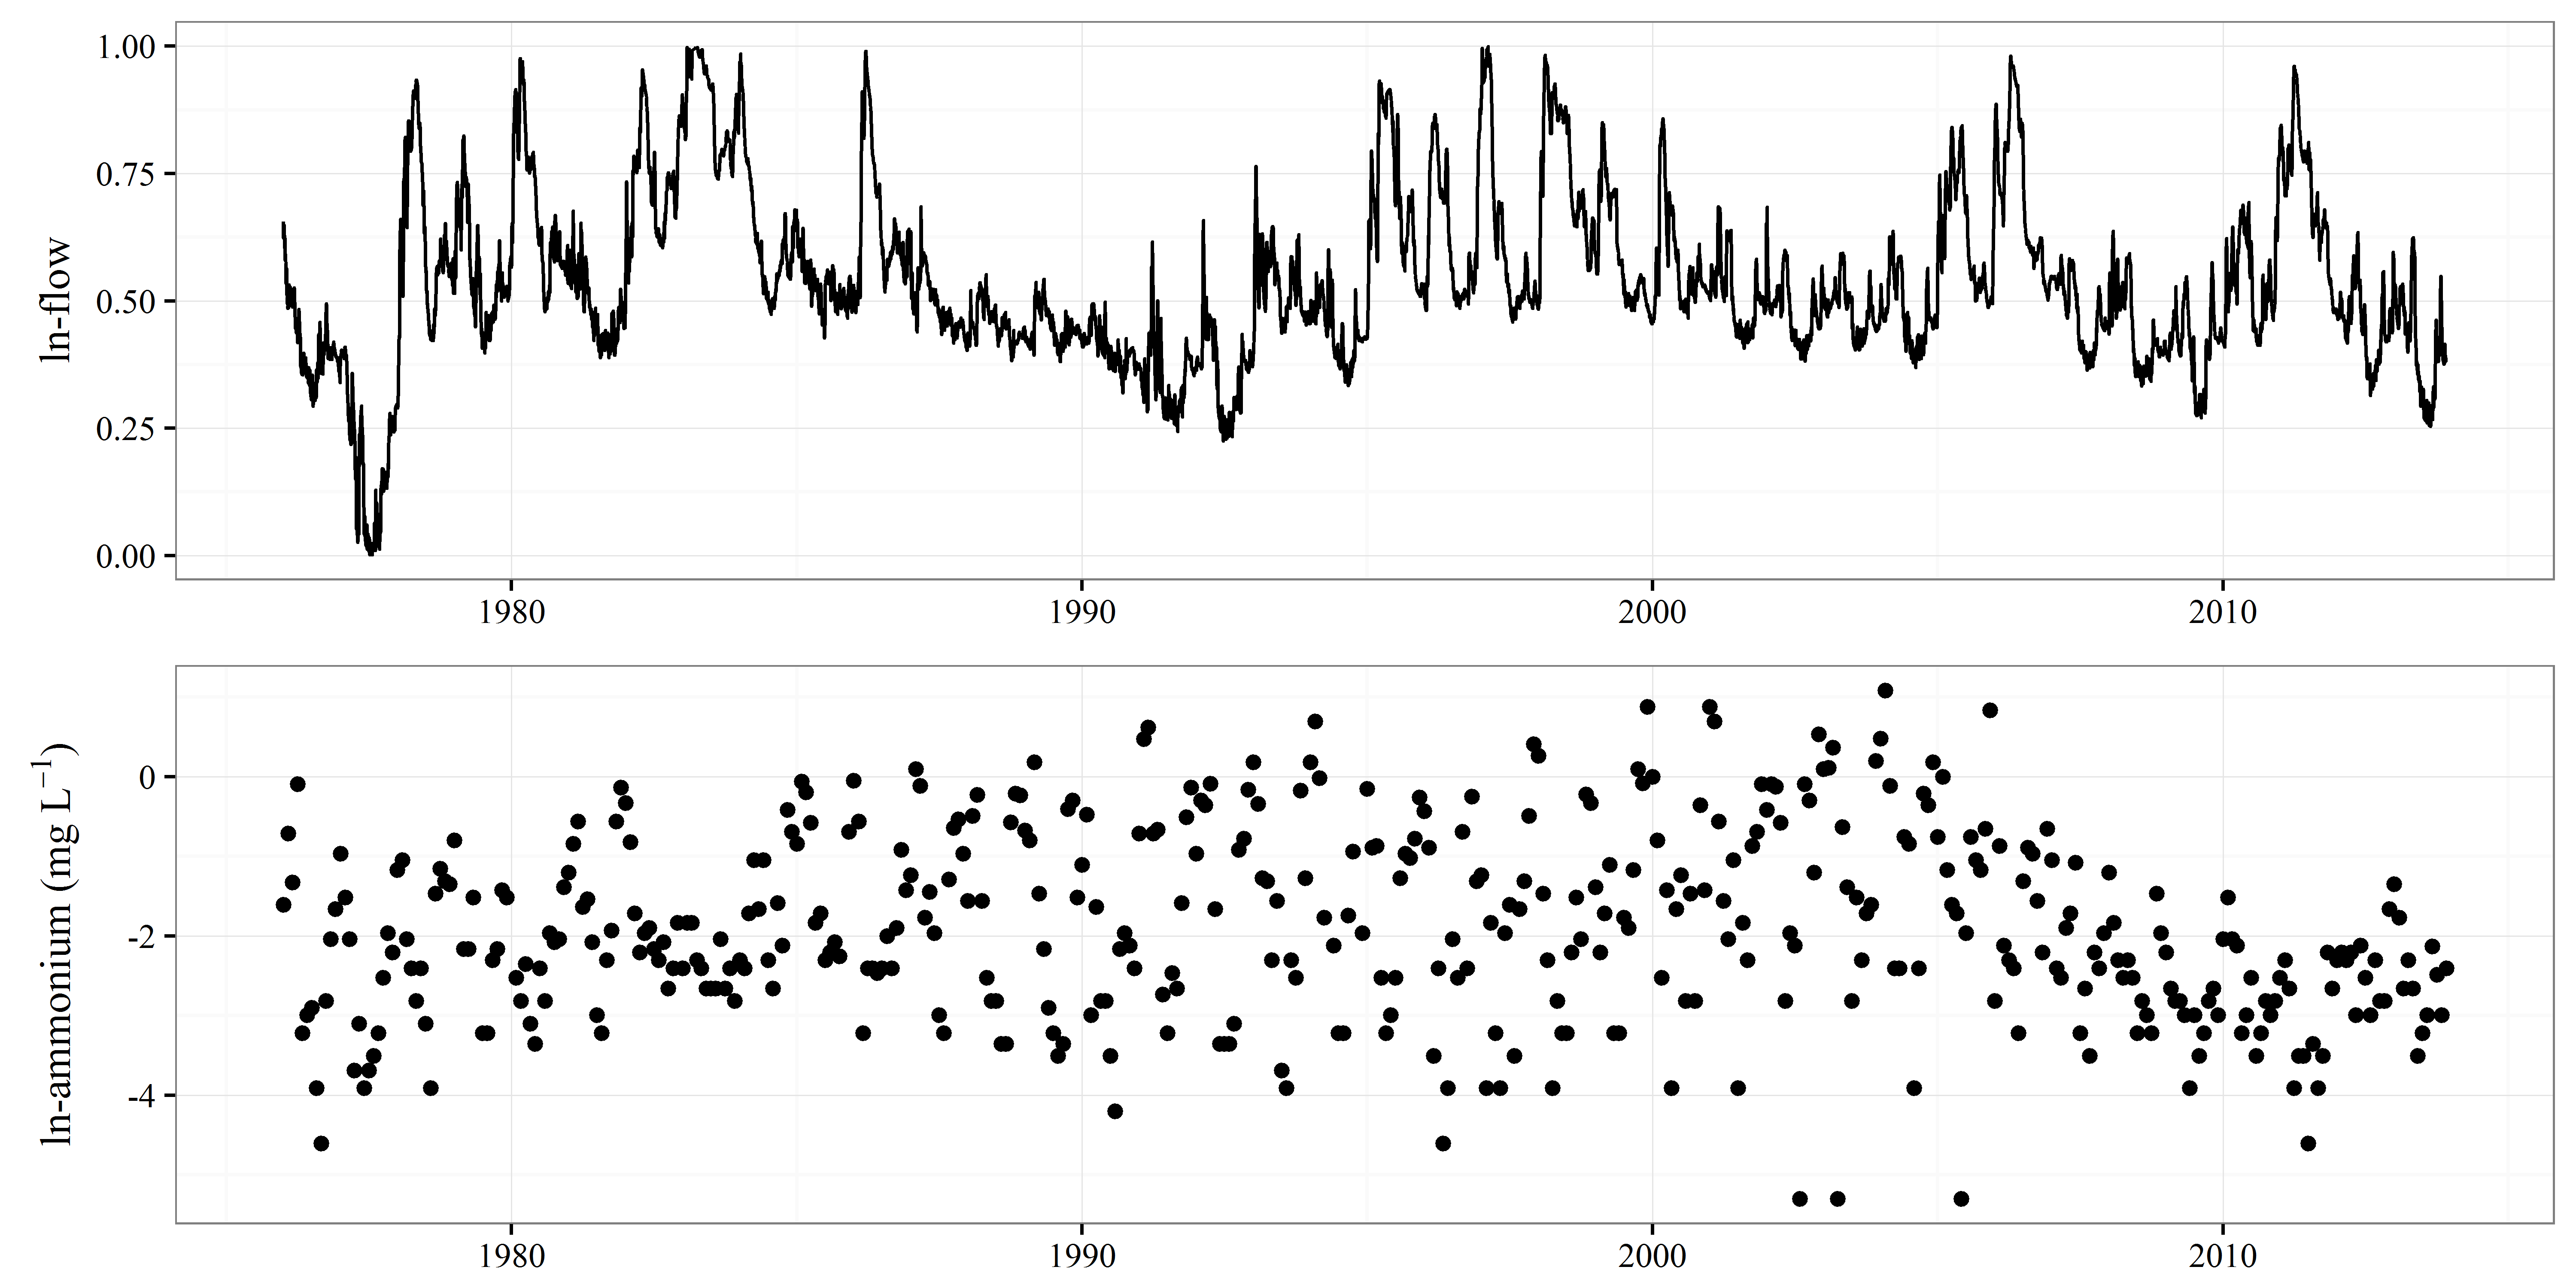
\includegraphics[width=\linewidth]{posterfigs/rawdat.png}}
      \caption{\footnotesize Example of flow data (top) and nitrogen data (bottom) at C10 used for trend analysis.}
	    \end{figure}		
	    \end{column}
	    
	    \begin{column}{0.45\linewidth}
	    test
	    \end{column}
	    
	    \end{columns}
	    
      \end{block}

   		%%%%%%
			% Second Objective
			%%%%%%
      \begin{block}{Trend Analyses}
				
			\end{block}

    \end{column}
 
  \end{columns}

\end{frame}

\end{document}
